
\chapter{Haskell-Python}
\label{chap:hs}

Haskell-Python is an interpreter for a language similar to Core, we call it Core' here.
This interpreter is the base for our JIT compiler. In this chapter we descripe a 
syntax and an informal semantics for Core'.

\section{Syntax}
\label{sec:syntax}

Although Core' does not have a syntax, we define one here, as we use it later 
to show how Core is translated to Core'.

In the following grammar, the '[' and ']' symbols are used to mean that
anything between can be repeated, 0 or more times. We use '[' and '$]^+$' to 
mean that the pattern can be repeated 1 or more times. Non-terminals are 
written with italic font throughout the paper.
\\
\\
\begin{grammar}

<constructor> ::= c( <symbol> [ <value> ] )

<function> ::= f( <symbol> [ <rule> ]$^+$ )

<rule> ::= r( [ <value> ]$^+$ = <exp> )

<exp> ::= e( <value> )
     \alt e( <primitive-function> )
     \alt e( <function> )
     \alt e( <application> )

<application> ::= a( <exp> [ <value> ] )

<value> ::= <literal>
       \alt <constructor>
       \alt <variable>

<literal> ::= l( <string> )
	 \alt l( <number> )
	 \alt l( <character> )

<symbol> ::= A symbol is just a string-identifier.

<string> ::= A list of characters

<number> ::= A number

<character> ::= A character

<primitive-function> ::= A function that can't be defined in terms of other functions.

\end{grammar}


\section{Informal semantics}

The Launchbury semantics is an operational semantics for 
lazy evaluation, which the Core' interpreter follows rather closely. 
This section will be a brief introduction to the semantics of the interpreter.
For a introduction to 
the Launchbury semantics, see \cite{launchbury1993natural}. 

A Core' program is evaluated by reducing the main application to WHNF 
(Weak Head Normal Form). A construct is in WHNF if it can't be
reduced any further.

\subsection{Value}
A value can be a literal, constructor, or a variable. All values are in WHNF.

\subsection{Constructor}
A constructor is just a value, containing other values.

\subsection{Function}
A function is a named collection of rules. It must contain at least one rule.

\subsection{Rule}
A rule is a list of values, followed by an expression. Note that the only variables
that are in scope in the expression, are those defined in the list of values.

\subsection{Expression}
An expression can be a value, a primitive-function, a function, or an application.
An expression is in WHNF if it does not contain any unevaluated applications.

\subsection{Application}
An application represents the evaluation of a function with variables applied to it.
An application is not in WHNF.

When the application is evaluated, the arguments are matched against the list of 
values contained in the list of rules. 
When the arguments match a rule, the expression contained in this rule is evaluated. 
The variables in the expression are replaced by the values that matched the same-name
variables in the value list. Then the expression is evaluated, returning a new value.

\subsection{Literal}
A literal is a value such as an integer, a string or a character.


\section{Evaluation}

A Core' program is executed by reducing a main Application to WHNF.

\subsection{The evaluation stack}

When an Application is evaluated; two things can happen. If it does not contain
other unevaluated Applications it can be evaluated directly. However, if it does
contain unevaluated Applications, it is turned into a Thunk (a suspended evaluation)
untill its unevaluated parts have become evaluated (reduced to WHNF).

When a Thunk is created, it is pushed onto the evaluation stack, and its 
unevaluated parts are pushed ontop of it. Since evaluation is proceeded from the
top of the stack, this ensures that when the Thunk is reached, its applications
have been evaluated.

%it's unevaluated parts is pushed onto an 
%evaluation stack. The stack can contain two kinds of elements, a CopyStackElement,
%and a UpdateStackElement. Evaluation is always continued from the head of the stack.

% An UpdateStackElement contains a Thunk. ?

% A CopyStackElement contains an Application. ?

%\subsection{Thunk}

%A Thunk is a suspended evaluation, in effect, an unevaluated function application.

\section{Implementation}

The description of Haskell-Python can be 
logically divided into two parts; "the way programs are 
represented", and "the way programs are evaluated".

\subsection{Program representation}

Programs are represented by a set of Classes; Value, Constructor, Function, Rule, 
PrimFunction, Var, Application (Additional classes are created for Constructor
and Application for various number of arguments through the classes ConstructorN 
and ApplicationN). The syntax defined in \ref{sec:syntax} corresponds very much
to the organization of classes in the interpreter. See figure \ref{fig:classdia} 
for a full class diagram of the interpreter.

A Value is a base class for objects in WHNF. A Constructor inherits from Value.
The Function and PrimFunction also inherits from Value (indirectly 
via inheritance of AbstractFunction). Functions are Values because they can't 
be reduced any further (they are already in WHNF).

% Can a constructor contain all HaskellObjects ??? Why ?
The Constructor classes can contain Values as their arguments, however, since
a Constructor is itself a Value, it can not have unevaluated applications as
arguments. The Constructor is characterized by a Symbol. A Symbol is simply
a name that can be matched by identity.

The PrimFunction class represents a function that is not implemented in 
Haskell, but is implemented at the machine level.

The Function class represents a user-defined function.

A Var is substituted with a NumberedVar when a Rule is created. This simply
means that the new NumberedVar is only in scope within the Rule.

\subsection{Program evaluation}

A Substitution is the body of a Function with numbered variables 
(NumberedVar) substituted by values.

The evaluation of a program is done by a function, main\_loop. The function
takes a variable 'expr' as argument, and reduces it to WHNF. The reduction is done
by continously pushing/popping from the evaluation stack. 

The evaluation stack is represented by a base class, StackElement. Two other
classes inherits from this class, UpdateStackElement and CopyStackElement. Note that
the stack is implemented by a linked list (each StackElement points to the next).

% TODO ! Describe how recursion works in this same way.
\begin{figure}[H]
\centering
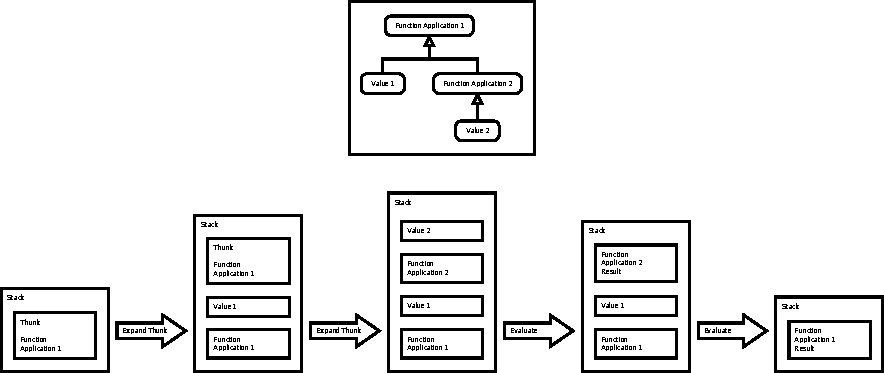
\includegraphics[width=\textwidth]{../diags/eval-stack.pdf}

\caption{Overly simplified concept sketch of the evaluation stack; 
Nothing will be done to Value 2, it is
in WHNF. The point is, that by the time we get to Function Application 2, we can be
sure that all its arguments have been evaluated. And when we reach Function Application 1,
the same can be said for it.}
\label{fig:classdia}

\end{figure}


\begin{sidewaysfigure}
\begin{figure}[H]
\centering
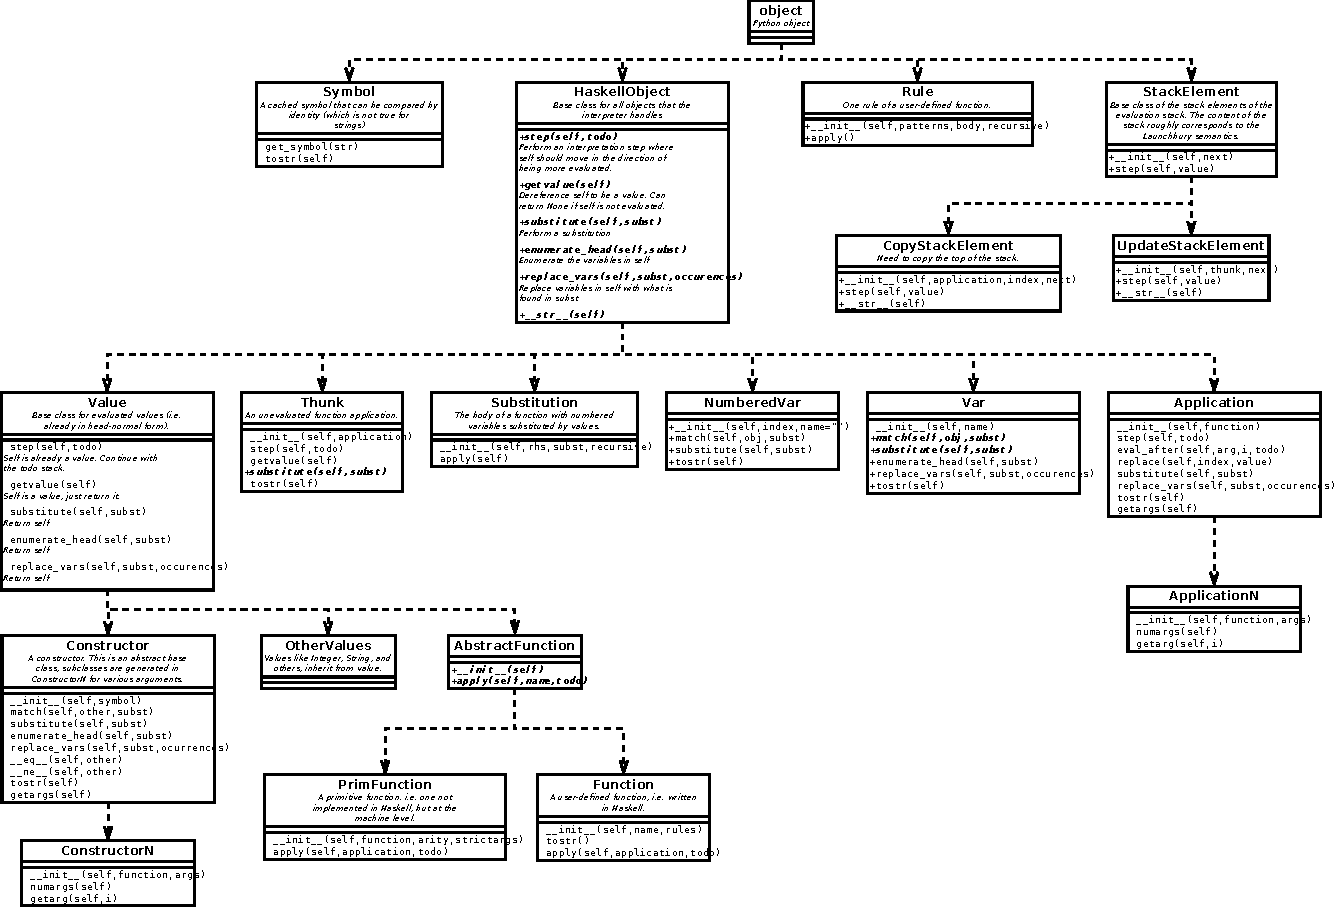
\includegraphics[angle=270, width=\textheight]{../diags/core-interp.pdf}

\caption{Haskell-Python class diagram}
\label{fig:classdia}

\end{figure}
\end{sidewaysfigure}

\section{Extensions}

\subsection{GHC usage}

% TODO

By using GHC to compile the Haskell programs and dump its intermediate
format to a file, we can effectively turn Haskell-Python into a full
Haskell compiler. However, the format dumped by GHC is external-core.

We turn external-core into JSCore with a Haskell program called core2js.
JSCore is a JSON compliant representation of external-core. This means that
we can parse JSON and get a representation we can easily traverse when building
the AST (Abstract Syntax Tree) for the Core' interpreter.

\subsection{Module system}

% TODO
...

\subsection{Parser}

% TODO
...  See chapter \ref{chap:rewrite} for a detailed description of the parser.

\subsection{Primitives}

% TODO
...
